\chapter{Suchalgorithmen}
\section{Systematische Suche}
Ein rationaler Agent sieht die Welt in verschiedenen Stati, z.B. wären da der aktuelle Zustand und der Zielzustand der Welt. Der rationale Agent muss jetzt eine Folge von Aktionen finden, welche ihn vom Initialzustand in den Zielzustand bringt.
\subsection{Voraussetzungen für eine Suche}
Ein rationaler Agent ist in den Ferien und muss so schnell wie möglich von Arad nach Bukarest , da dort sein Flieger geht. Wie schafft er das? Mit der Suche eines schnellstmöglichen Weges. \\ \newline
Generell kann man sagen, dass wenn die Umwelt folgende Eigenschaften erfüllt, der Agent eine \textbf{Sequenz von Aktionen} suchen kann, welche ihn zum Zielzustand führen werden:

\begin{enumerate}
	\item \textbf{Observable} - Der Agent weiss, wo er ist.
	\item \textbf{Static} - Die Umwelt verändert sich nicht plötzlich.
	\item \textbf{Deterministic} - Jede Aktion hat den gewünschten Effekt.
	\item \textbf{Discrete} - Nur eine finite Anzahl von Aktionen ist möglich in jedem Zustand.
\end{enumerate}

Im Beispiel Arad nach Bukarest sind diese Eigenschaften gegeben. Der Agent weiss, wo er sich befindet, die Städte verändern nicht plötzlich den Ort, und wenn er von einer Stadt in die nächste fährt, dann fährt er auch dorthin. Und, gegeben die Abstraktion, er kann nicht unendlich viele Städte direkt erreichen. Ein Status wäre hier z.B. die aktuelle Stadt auf der Karte, die Aktionen die Reise zwischen den Städten - also die Kanten des Graphen, die Aktionskosten die Distanz-Informationen auf den Kanten. 

\begin{figure}[h]
\centering
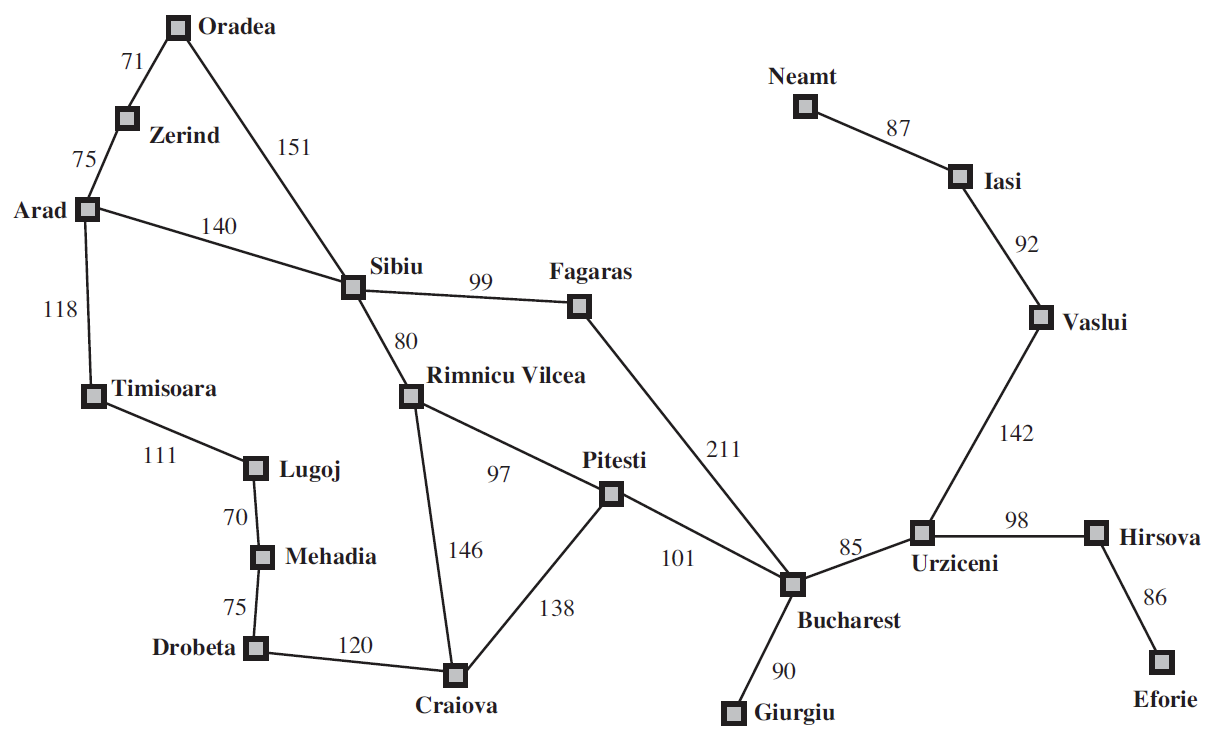
\includegraphics[width=0.5\linewidth]{fig/travel_example}
\caption{Beispiel für eine Umgebung wo eine Suche möglich ist}
\label{fig:travel_example}
\end{figure}

\subsection{Begrifflichkeiten}
\begin{description}
	\item[Initial State] Der erste Status des Agenten
	\item[State Space] Alle möglichen Stati (z.B. der Graph aller Städte)
	\item[Actions] Alle möglichen Aktionen
	\item[Transition Model] Eine Funktion, welche as Input einen Status und eine Aktion hat, und daraus einen neuen Status generiert. z.B. \texttt{succ(Arad, (Arad-Sibiu)) = Sibiu}.
	\item[Goal Test] Sind wir schon da? Sind wir schon da?
	\item[Path] Die Sequenz der Aktionen.
	\item[Path Costs] Die Kostenfunktion über den Gesamtpfad. Meistens die Summe der Kosten aller Einzelaktionen, aber z.B. bei einer Aktion 3 für 2 wäre es wieder anders.
	\item[Solution] Pfad vom Intialzustand zum Zielzustand.
	\item[Optimal Solution] Pfad vom Initialzustand zum Zielzustand mit den niedrigsten Kosten.
	\item[Search Costs] Die Kosten (Zeit \& Speicherverbrauch) um eine Lösung zu finden.
\end{description}

\subsection{Beispielmodelle}
\subsubsection{8 Puzzle}
\begin{figure}[h!]
\centering
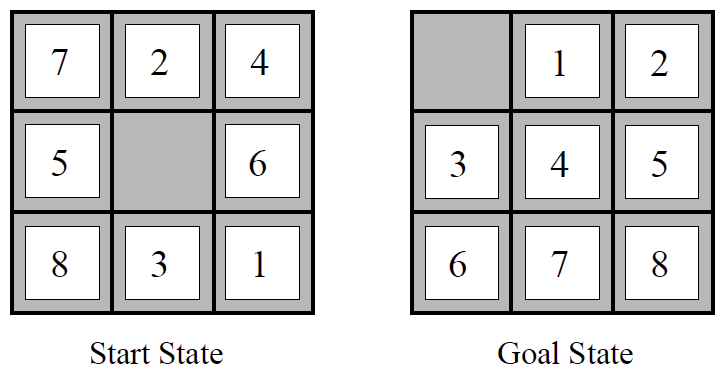
\includegraphics[width=0.6\linewidth]{fig/8_puzzle}
\caption{Das Spiel 8 Puzzle}
\label{fig:8puzzle}
\end{figure}

In diesem Spiel wäre der aktuelle Status die Position der Spielsteine. Die Aktionen wären \textit{bewege das leere Feld} (simpler als die anderen zu bewegen) und der Goal Test wäre dann einfach \textit{ist der Zielzustand = aktueller Zustand}. Die Pfadkosten, sind hier definiert als jede Aktion kostet 1.

\subsubsection{8 Queens}
In diesem Spiel geht es darum, 8 Damen auf einem Feld so zu platzieren, dass keine Dame eine andere Dame bedroht. Hier ist der Zielzustand im Vorfeld unbekannt.
\begin{figure}[h!]
	\centering
	\begin{subfigure}[h]{0.2\textwidth}
	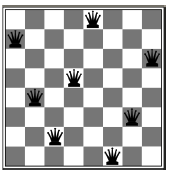
\includegraphics[width=\textwidth]{fig/8_queens_end}
		\caption{Zielzustand 1}
	\end{subfigure}
	~
	\begin{subfigure}[h]{0.2\textwidth}
	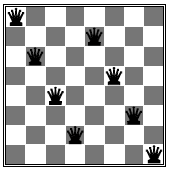
\includegraphics[width=\textwidth]{fig/8_queens_start}
		\caption{Zielzustand 2}
	\end{subfigure}
	\caption{Mögliche Zielzustände}
\end{figure} 

Der aktuelle Status wäre wieder die Position der Damen auf dem Brett, der Initialstatus wäre ein leeres Brett, die \textit{Successor function}, dass man eine Dame zum Brett hinzufügt, und der Goal Test ist auch klar - es sind 8 Damen auf dem Brett die sich nicht bedrohen. Die Pfadkosten sind hier eigentlich egal, wir sind ja nur an der Lösung interessiert.

Optimaler wäre die Sucessor Function so zu definieren, dass man die Damen einfach Spaltenweise hinzufügt.

\subsection{Suchbaum}
\begin{figure}[h!]
	\centering
	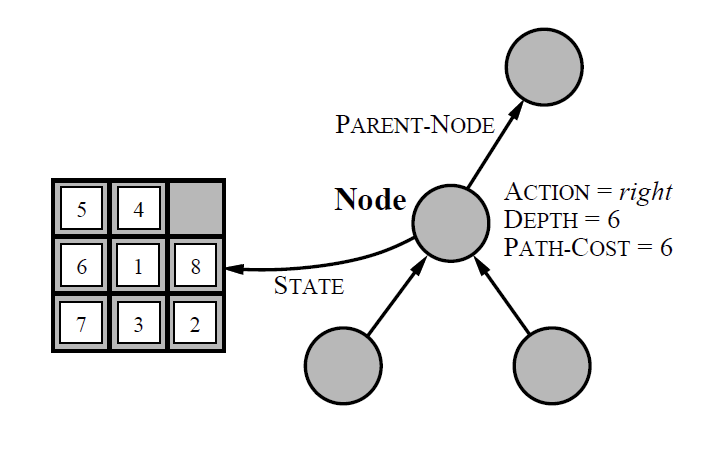
\includegraphics[width=0.5\linewidth]{fig/search_tree}
	\caption{Suchbaum Aufbau}
	\label{fig:search_tree}
\end{figure}
Ein Suchbaum beschreibt die Reihenfolge, in der Knoten im Suchraum besucht werden. Ein Knoten beschreibt dabei einen Status, die letzte Aktion, die zu ihm geführt hat (denn Status + Aktion = Status) und die aktuellen Pfadkosten. Er hat verschiedene Kinder, welche durch entsprechende Aktionen erreicht werden können.
\begin{description}
	\item[Frontier] Die Knoten, welche gerade von der Suchfunktion gefunden wurden und die noch nicht weiter untersucht werden.
	\item[Repeated State] Stati, welche im aktuellen Suchbaum schonmal vorkamen.
	\item[Redundant Paths] Wenn 2 Pfade gefunden werden, welche zum selben Status gelangen.
	\item[Search Space] = Suchraum. Ein Graph, indem die Knoten alle Stati im \textit{State Space} darstellen und die durch entsprechende Aktionen verbunden sind.
	\item[Node expansion] Generiert alle Nachfolge-Knoten, gegeben die Aktionen.
	\item[Search Strategy] Bestimmt, welcher Knoten als nächstes expandiert / exploriert wird.
	\item[Tree-based Search] Suche bei der nur die Frontier gespeichert wird und die bereits besuchte Knoten immer wieder besuchen kann.
	\item[Graph-based Search] Suche bei der zusätzlich die besuchten Knoten ebenfalls gespeichert werden.
	\item[Dead End] Wenn bei einem Knoten keine unbekannten Kinder mehr vorhanden sind.
	\item[Explored Set] Ein Set aus besuchten Knoten. Wird nicht benötigt, wenn der Suchraum keine Schleifen enthält.
\end{description}

\subsection{Suchraum}
\begin{figure} [h!]
	\centering
	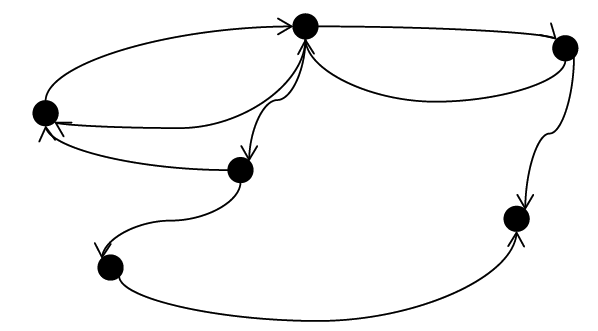
\includegraphics[width=0.2\linewidth]{fig/search_space}
	\caption{Beispiel für Suchraum 1}
	\label{fig:search_space}
\end{figure}

\begin{figure} [h!]
	\centering
	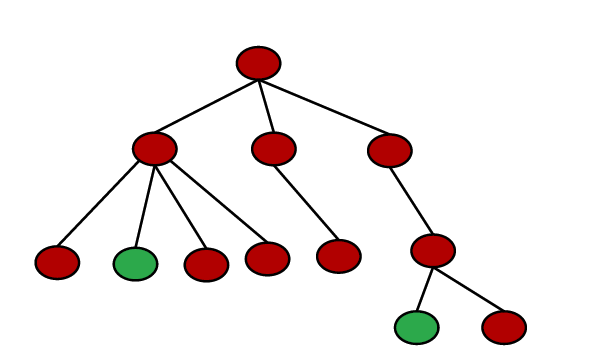
\includegraphics[width=0.2\linewidth]{fig/suchraum}
	\caption{Beispiel für Suchraum 2}
	\label{fig:suchraum}
\end{figure}

Dieser Suchraum in Abbildung \ref{fig:suchraum} hat bestimmte Eigenschaften.
\begin{description}
	\item[b] Branching Factor - max. Anzahl Kinder eines Knotens - hier \textbf{4}
	\item[d] Depth of shallowest goal - hier wäre die Tiefe des ersten grünen Knotens \textbf{2}.
	\item[m] Maximum Length - Maximale Pfadlänge - hier \textbf{3}.
\end{description}

\subsection{Breadth-First Search (BFS)}
Hier wird zuerst in die Breite gesucht. Das heisst, dass wenn ein Knoten gefunden wird, wird er in eine FIFO Queue gesteckt, welche dann nacheinander abgearbeitet wird.
\begin{figure} [h!]
	\centering
	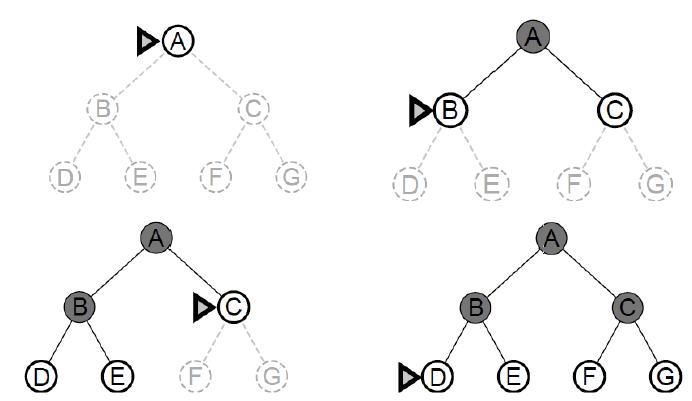
\includegraphics[width=0.4\linewidth]{fig/bfs_search}
	\caption{Breadth-First Search}
	\label{fig:bfs}
\end{figure}
BFS findet alle Lösungen und wenn die Aktionen alle dieselben positiven (oder null) Kosten haben, dann findet es auch die optimale Lösung. Es findet ja immer die Lösung, die am wenigsten tief im Baum vorhanden ist.
\subsubsection{Zeitbedarf \& Zeitkomplexität}
Ein BFS Suchbaum muss ja bis zur Tiefe des Lösungsobjekt komplett aufgebaut werden. Wenn \textbf{b} der \textit{branching factor} ist und \textbf{d} die Tiefe der Lösung heisst das, dass diese Anzahl an Knoten besucht werden müssen:

\begin{displaymath}
	\displaystyle\sum_{i=1}^{d} b^i = b + b^2 + b^3 + \dots + b^d \approx O(b^d)
\end{displaymath}

\subsubsection{Speicherbedarf \& Speicherkomplexität}
BFS speichert offenbar jeden besuchten Knoten ab, da der Pfad zur gefundenen Lösung ja auch bekannt sein muss. Daher ist der Speicherbedarf, gleich wie der Zeitbedarf:

\begin{displaymath}
\displaystyle\sum_{i=1}^{d} b^i = b + b^2 + b^3 + \dots + b^d \approx O(b^d)
\end{displaymath}
Die Frontier hat \(O(b^d)\) und das explored set \(O(b^{d-1})\).

\subsection{Depth-First Search (DFS)}
Die Depth First Search ist ähnlich wie die Breadth-First Search. Die gefundenen Knoten werden hier aber in eine LIFO Queue gesteckt. Das bewirkt, dass zuerst in die Tiefe gesucht wird und erst dann schrittweise in die Breite.
\begin{figure} [h!]
	\centering
	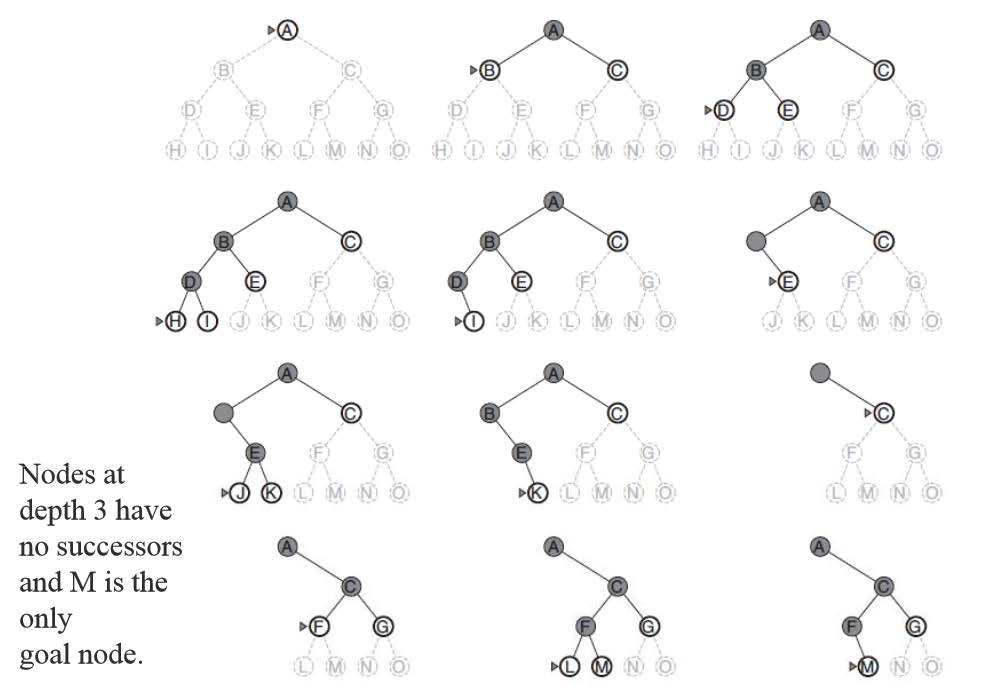
\includegraphics[width=0.7\linewidth]{fig/dfs_search}
	\caption{Depth-First Search}
	\label{fig:dfs}
\end{figure}
DFS ist keine optimale Suche, es kann sein dass eine Lösung tief unten 'vergraben' liegt, und wenn sie dann unendlich tief ist, geht sie dort natürlich auch suchen. Wenn die besuchten Knoten zusätzlich nicht gespeichert werden, dann kann sie auch für immer im Kreis herum suchen.
\subsubsection{Zeitbedarf \& Zeitkomplexität}
Eine DFS Suche findet im schlechtesten Fall die Lösung erst wenn der ganze Baum durchsucht wurde. \textbf{m} heisst ja die maximale Tiefe und \textbf{b} wieder der \textit{branching factor.}

\begin{displaymath}
	b^m \approx O(b^m)
\end{displaymath}

\subsubsection{Speicherbedarf \& Speicheromplexität}
DFS muss nicht der gesamte Baum speichern, sondern nur der Pfad der gerade zum Objekt führt.

\begin{displaymath}
bm \approx O(bm)
\end{displaymath}
In Abbildung \ref{fig:dfs} sieht man das schön. Dort hat der Baum \(b=2, m=3\). In keinem Fall müssen also mehr als \(2*3=6\) Knoten gespeichert werden. \\ \newline
Wenn der Suchraum allerdings noch Schlaufen beinhaltet, so muss noch die besuchten Knoten gespeichert werden. Das kann bedeuten, dass im schlechtesten Fall der gesamte Baum abgespeichert werden muss.

\begin{displaymath}
b^m \approx O(b^m)
\end{displaymath}

\subsection{Depth-Limited Search (DLS)}
DLS ist DFS, einfach mit einem Limit wie tief die Suche gehen darf. Läuft jetzt nicht mehr unendlich, aber wenn die Lösung tiefer ist als das Limit wird sie natürlich nicht gefunden.
\subsubsection{Zeitbedarf \& Zeitkomplexität}
Gleich wie DFS, einfach anstatt Tiefe des Baums die Tiefe des Suchlimits. Das heisst Zeitbedarf ist jetzt (\textbf{l} = Limit)
\begin{displaymath}
b^l \approx O(b^l)
\end{displaymath}
\subsubsection{Speicherbedarf \& Speicheromplexität}
... und Speicherbedarf:
\begin{displaymath}
bl \approx O(bl)
\end{displaymath}

\subsection{Iterative Deepening Search (IDS)}
Wie DLS, einfach wird das Limit schrittweise angehoben. Ist also irgendwie eine Mischung aus BFS und DFS. Die ersten Schritte der Suche werden immer wiederholt. Es findet immer eine Lösung wenn eine da ist und ist sogar optimal, wenn die Kostenfunktion nicht abnimmt mit der Tiefe des Suchbaums.